We now provide a comprehensive view of the timescales that drive the interactions between nearest neighbors, as well as the times scale involved for the microstructure in buoyant homogeneous emulsions.

\tb{Start with the classic drift velocity plots And maybe the values of R}
\subsection{The relative velocity}

As it will be useful for scaling purposes we display on \ref{fig:Reall} the ensemble averaged \textit{Reynolds} number for all the DNS presented in this study.
Formally, we define this \textit{Reynolds} number As
\begin{align*}
    Re = \frac{\rho_f U d}{\mu_f} && \text{with}, && U = \textbf{u}_p - \textbf{u}_f
\end{align*}
where $\textbf{u}_f$ is the continuous phase velocity averaged over the volume occupied by this phase and over all simulation time. 
\begin{figure}[h!]
    \centering
    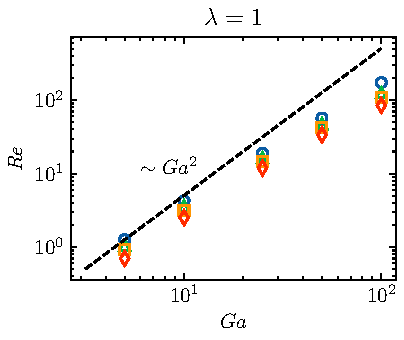
\includegraphics[height = 0.3\textwidth]{image/HOMOGENEOUS_NEW/CA/Re_l_1.pdf}
    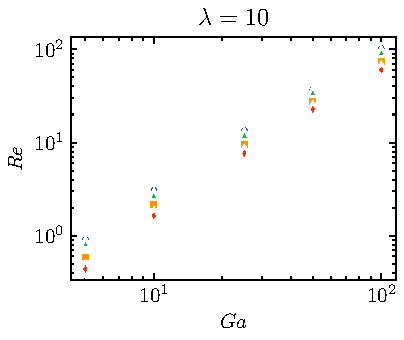
\includegraphics[height = 0.3\textwidth]{image/HOMOGENEOUS_NEW/CA/Re_l_10.pdf}
    \caption{
        Averaged Reynolds number based on the averaged drift velocity, $Re = \rho_fU d /\mu_f$, with $U = |\textbf{u}_p - \textbf{u}_f|$.
        $\textbf{u}_p$ and $\textbf{u}_f$ are the particle and fluid phase volume and time averaged velocity.
    }
    \label{fig:Reall}
\end{figure}
It is observed that for low $Ga$ the relative velocity scales approximately as $\sim Ga^2$, regardless of the volume fraction $\phi$ and viscosity ratio $\lambda$. 
It is expected that with a greater $Re$ we obtain more particle velocity fluctuations. 
As a result the particle time of interaction or the \textit{age}, is expected to be reduced with greater $Re$. 
Consequently, the \textit{random destruction assumption} discussed in \ref{sec:Theory} might be valid in this range of parameters. 
\begin{figure}[h!]
    \centering
    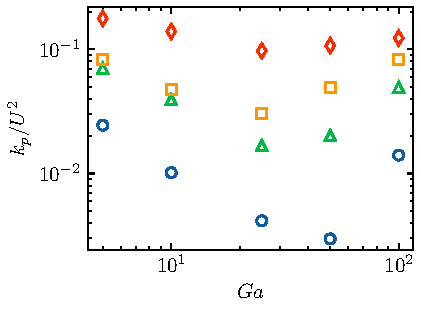
\includegraphics[height = 0.3\textwidth]{image/HOMOGENEOUS_NEW/PA/Talpha_l_1.pdf}
    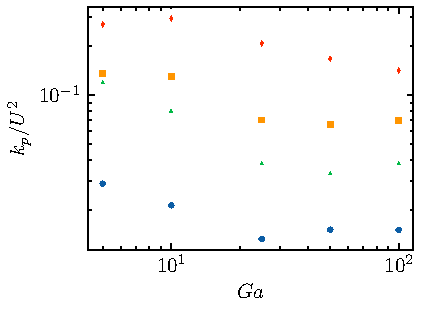
\includegraphics[height = 0.3\textwidth]{image/HOMOGENEOUS_NEW/PA/Talpha_l_10.pdf}
    \caption{
        Ensemble averaged dimensionless granular temperature $k_p = \frac{1}{2}\avg{\textbf{u}'_\alpha \textbf{u}_\alpha'}/U^2$.     
    }
    \label{fig:Reall}
\end{figure}

\subsection{Mean age of interaction}

Let evaluate the mean rate of destruction $1/\tau_p(\textbf{x},t)$ and verify the random destruction assumption via the study of $P_a(a)$.  


In \ref{fig:age_picture} (right) we display the dimensionless age distribution $P_a(a)$, measured in our DNS for different volume fraction at $\lambda =1$ and $Ga = 100$. 
The age is made dimensionless using the timescale, $U/d_p$ where $d_p = n_p^{-1/3}$.
Additionally, in \ref{fig:tau_p} we computed the mean first moment of the age distribution, which enable us to plot on \ref{fig:age_picture} the theoretical prediction for the age distribution $P_a(a)$. 
It is seen on \ref{fig:age_picture} (right) that the age distributions are rather well represented by the theoretical age distributions from \ref{eq:Pa}.
Consequently, the \textit{random destruction assumption} holds for these cases. 
\begin{figure}[h!]
    \centering
    % 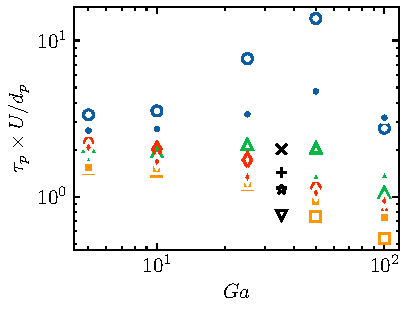
\includegraphics[height = 0.3\textwidth]{image/HOMOGENEOUS_NEW/tau_Ga.pdf}
    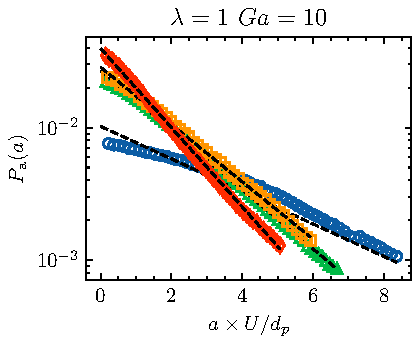
\includegraphics[height = 0.3\textwidth]{image/HOMOGENEOUS_NEW/Dist/Pa_l_1_Ga_10.pdf}
    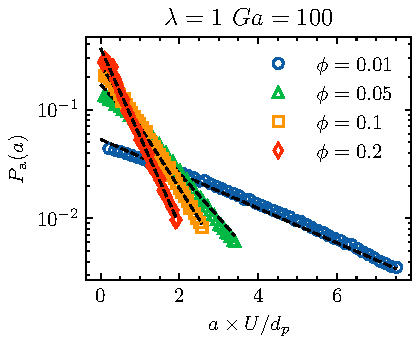
\includegraphics[height = 0.3\textwidth]{image/HOMOGENEOUS_NEW/Dist/Pa_l_1_Ga_100.pdf}
    \caption{
    Age distribution function $P_a(a)$ in terms of the dimensionless age, for $\lambda = 1$.
    (dashed lines) Theoretical age distributions, computed based on the mean age, see \ref{eq:Pa}. 
    The ages are made dimensionless using the relative velocity $U$ and the particle length scale $d_p = n_p^{-1/3}$.  
    (right) High inertia effects ($Ga = 100$),
    (left) Low inertia effects ($Ga = 10$),
    }
    \label{fig:age_picture}
\end{figure}
In \ref{fig:age_picture} (left)  we provided the age distributions for $Ga = 10$. 
It is seen that the age distribution is well represented by \ref{eq:Pa} for the dense emulsion ($\phi \le 0.05$).
However, for $\phi = 0.01$ we observe that the predicted values of $P_a$ is higher than the DNS results for small ages and smaller for high ages. 
Therefore, at low \textit{Galileo} and low $\phi$ the \textit{random destruction assumption} doesn't seem to remain valid. 
As mentioned earlier the \textit{random destruction assumption} must hold true for flows with high particle velocity fluctuations, since it induces randomness among the particle interactions \citep{zhang2023evolution}. 
It is clear that for $\phi \to 0$ and $Re \to 0$, the particle phase fluctuation also tends to $0$, making this condition harder to meet. 
Additionally, no particular differences on $P_a$ is observed when $\lambda = 10 $ therefore we do the display the graphs. 
Apart from the dilute and low inertia cases, it is reasonable to say that \ref{eq:Pa} is well representative of the age distribution function with DNS.
Consequently, averaged inverse rate of destruction $\tau_p$, is equivalent to the mean particle interaction time for most of the cases considered here.  


\begin{figure}[h!]
    \centering
    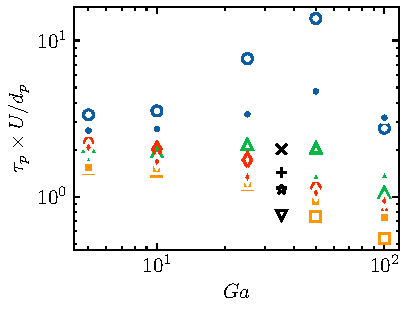
\includegraphics[height = 0.3\textwidth]{image/HOMOGENEOUS_NEW/tau_Ga.pdf}
    % 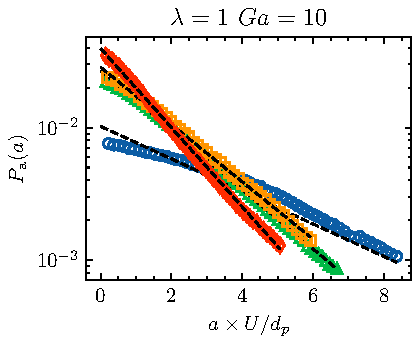
\includegraphics[height = 0.3\textwidth]{image/HOMOGENEOUS_NEW/Dist/Pa_l_1_Ga_10.pdf}
    % 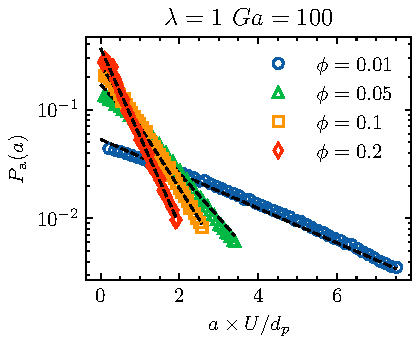
\includegraphics[height = 0.3\textwidth]{image/HOMOGENEOUS_NEW/Dist/Pa_l_1_Ga_100.pdf}
    \caption{
    (left) Mean dimensionless age $\tau_a =  \int_0^\infty aP_a(\textbf{x},t,a)da$ in terms of the \textit{Galileo} number for different volume fraction :   
    ($\pmb\bigcirc$) $\phi = 0.01$; ($\pmb\triangle$) $ \phi = 0.05$; ($\pmb\square$) $\phi = 0.1$ ($\pmb\lozenge$) $\phi = 0.2$.
    The hollow symbols correspond to $\lambda = 1$, the filled symbols to $\lambda = 10$.
    Black symbols represent the DNS results of \citet{zhang2023evolution} for hard sphere suspension with $\phi = 0.0168,0.0565,0.1341,0.2622$, corresponding to the symbols : $\pmb\times, \pmb +, \pmb\star , \pmb\triangledown$, respectively.
    }
    \label{fig:tau_p}
\end{figure}
In \ref{fig:tau_p} we displayed the dimensionless mean age for all our numerical experiment. 
Let first comment the non-dilute cases $\phi\geq 0.05$. 
It seems that $\tau_p$ is well scaled by $U/d_p$ for this range of volume fraction since its values range between $2$ and $0.5$, which is reasonably close to $1$. 
At low volume fraction it might be observed that $\tau_p$ is independent of $Ga$, then for $Ga > 50$ it start to decr
% Regarding the global trend of $\tau_p$, we can say that for almost all of our DNS, the time of interaction is higher for $\lambda = 1$ (hollow symbols) than for $\lambda = 10$ (filled symbols) at same $Ga$ and $\phi$.

At low volume fraction however, $\tau_p$ is clearly higher and reaches a peak at $\phi=0.01$, $Ga=50$, $\lambda=1$.
This, may be correlated with the values of $A_{xx}$ on \ref{fig:A} which also reach a maximum for these parameters. 
Indeed, since $A_{xx}$ is rather high for these simulations, we know that particles are, on average, in a side-by-side configuration, which seems to be a stable configuration since $\tau_p$ is large too.
For $\lambda = 10$ we observe a smaller $\tau_p$ and a smaller $A_{xx}$ at $\phi = 0.01$ and $Ga = 50$, indicating that, on average, the interaction are not as long, while the microstructure is more isotropic. 
The dilute suspension of hard spheres, represented by a $\pmb\times$ symbol, seems to possess even lower $\tau_p$. 
This suggests that solid particles do not necessarily reach a stable equilibrium configuration in the dilute regime, unlike the bubble-like particles ($\lambda = 1$). 
This observation might be explained by the generation of more vorticity in the wake of viscous and solid particles, which makes the interactions less stable at these $Ga$ and $\phi$ values.
These pair interactions mechanisms have been investigated by \citet{yin2008lattice} when studying spherical bubbles and solid particles suspensions.
They reach the conclusion that the weaker wake generated by bubbles tends to make them spend more time in close horizontal orientations, in opposition to solid spherical particles. 
This finding strongly support the previous hypothesis. 
In summary, the mean age of interaction seem to be a good way to measure the particles pairs stability, since it provide a way to measure their interaction time. 
This time is shorter for increasing $\phi$, $\lambda$ and $Ga$, if $\phi \neq 0.01$ in which case it is non-monotonic with $Ga$. 

\tb{AT this point include the DEATH rate }
As mentioned above, $\tau_p(\textbf{x},t)$ is the relaxation time of $\textbf{R}(\textbf{x},t)$. 
Consequently, the microstructure relaxation of dilute suspensions is larger, especially at $Ga = 50$, and may need a consequent amount of time to reach a steady state regime. 
This implies that the terms on the left-hands side of \ref{eq:dt_R} may not be neglected and that direct closure for the microstructure in terms of $\phi$, $Ga$ and $\lambda$ may not be achievable at these large $\tau_p$. 
In turns, this relaxation time will be reflected on the drift velocity between both phases, which is microstructure dependent. 
\begin{figure}
    \centering
    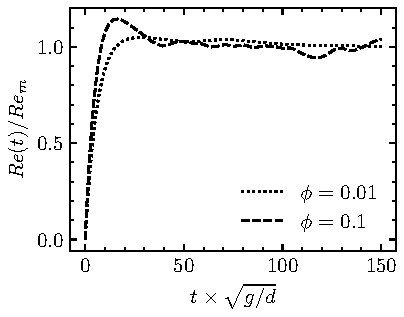
\includegraphics[height=0.325\textwidth]{image/HOMOGENEOUS_NEW/CA/Relax2.pdf}
    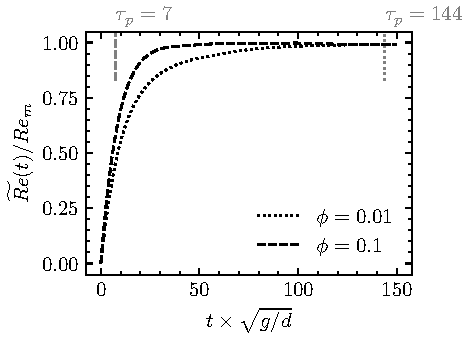
\includegraphics[height=0.35\textwidth]{image/HOMOGENEOUS_NEW/CA/Relax.pdf}
    \caption{
        (left) Average of the Reynolds number based on the instantaneous volume averaged drift velocity, $Re(t) = \rho_fU d /\mu_f$, with $U(t) = |\textbf{u}_p - \textbf{u}_f|$, divided by the mean Reynolds number $Re_m$ in terms of the dimensionless time. 
        (right) Running average of the Reynolds number $\widetilde{Re}(t)$ divided by the mean Reynolds number.
        For $\lambda = 1$ and $Ga = 50$ and two volumes fraction. 
        $\textbf{u}_p$ and $\textbf{u}_f$ are the particle and fluid phase volume averaged velocity at time $t$.
        The verticals gray lines indicate the values of $\tau_p$ all cases. 
        }
        \label{fig:relax}
\end{figure}
Indeed, in \ref{fig:relax} (right) we display the running average of the Reynolds number, based on the drift velocity, divided by the mean Reynolds number of the simulation for two values of $\phi = 0.01,0.1$ at $Ga = 50$ and $\lambda =1$. 
% It is seen that time, at which the simulation reaches a steady state regime is correlated with $\tau_p$. 
In this case we assume that two timescales are involved to bring the drift velocity to its statistically steady state regime. 
The first one is the particles' timescale, which is the time taken for a single particle to reach its own terminal velocity. 
The second timescale is the time taken for the microstructure to go from random, to its steady state microstructure. 
As a matter of fact, on \ref{fig:relax} we see that in the dilute regime ($\phi=0.01$) the rising velocity reaches its averaged value, at a time roughly equal to $100\sqrt{g/d}$ which is of the same order of magnitude than $\tau_p = 144\sqrt{g/d}$. 
On the contrary, when $\phi =0.1$ the averaged Reynolds number is indeed reached earlier ($t = 30\sqrt{g/d}$), despite the higher velocity fluctuations present in this case, see \ref{fig:relax} (left). 
The particle timescale is the same for both cases displayed \ref{fig:relax}, since only the volume fraction changes.
Additionally, the Statistical samples are supposed to be equivalent at same time since each  case posses the same number of droplets per domain. 
Thus, the changes in relaxation time is solely due to the microstructure relaxation timescale. 
Therefore, in support of the theory, $\tau_p$ seems capable of predicting the relaxation time of the microstructure.


The rising velocity of particles is directly correlated to the interphase drag force in sedimentation problems \citep{jackson1997locally}. 
Therefore, in the objective of finding closure terms for the averaged models, one must perform DNS for a time longer than $\tau_p$ plus the particle timescale, to allow the microstructure to relax adequately.
Then by performing an ensemble average procedure, one is able to build drag force models. 
Once established, these models will remain valid only under the condition where the timescale of the macroscopic flow significantly exceeds $\tau_p(\textbf{x},t)$ plus the particle timescale.
Indeed, these models have been built for relaxed microstructure and can be utilized only in this context.
Consequently, $\tau_p$ among other factors such as the particle relaxation time, provides a threshold value for the timescale not achievable in Euler-Euler models. 

\subsection{Particles normal approach velocity}

\tb{je ne suis plus tellement sur de la pertinience de cette section}

In the next section we will be interested in the velocity fields $\textbf{w}_p^\text{nst}$ since it appear in the source term $\textbf{W}(\textbf{x},t)$, which is at the origin of the modifications of the microstructure, see \ref{eq:dt_R}. 
To give a simpler representation of $\textbf{w}_p^\text{nst}$, we first study the normal approach velocity averaged on all $\textbf{r}$, that is,  
\begin{equation*}
    w_{pn}^aP_a(\textbf{x},t,a)
    = \frac{1}{n_p(\textbf{x},t)}
    \int_{\mathbb{R}^3}
    \frac{\textbf{r}}{r} \cdot \textbf{w}^\text{nst}_p
    P_\text{nst}(\textbf{x},\textbf{r},t,a) d\textbf{r}.
\end{equation*}
In this way, $w^\text{a}_{pn}(\textbf{x},t,a)$ is the average relative normal approach velocity between the nearest pair of particles at age $a$. 
The superscript $^a$ indicate that $w_{pn}^a$ is conditioned only on the age $a$. 
It represents the average approach velocity from one particle to its nearest neighbor, measured from the time when the particles became nearest neighbors, $a=0$.
A scheme of what $\frac{\textbf{r}}{r} \cdot \textbf{w}^\text{nst}_p$ is,  is given \ref{fig:normal_vel_picture} (right). 
\begin{figure}[h!]
    \centering
    % 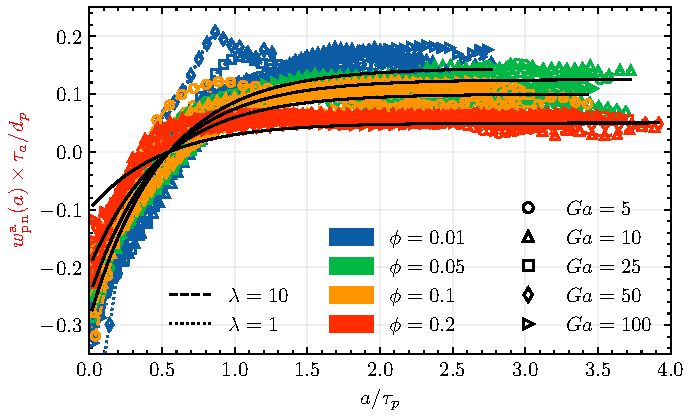
\includegraphics[height = 0.4\textwidth]{image/HOMOGENEOUS_NEW/Age_cond/uR_rel.pdf}
    % \includegraphics[height = 0.3\textwidth]{image/HOMOGENEOUS_NEW/Age_cond/r_l_10_PHI_10.pdf}
    \begin{tikzpicture}[ scale = 0.6]
        \node (img) at (-0.7\textwidth,0){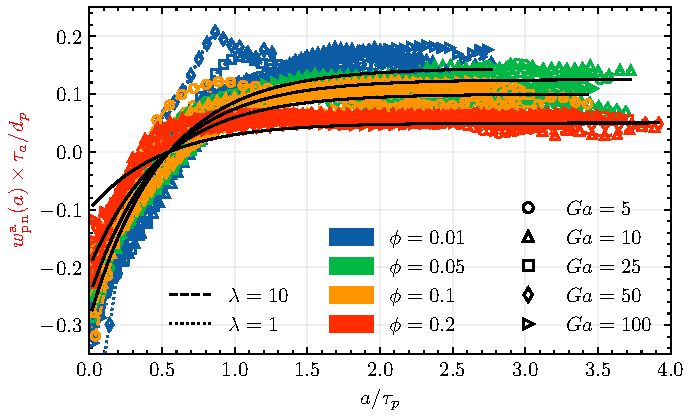
\includegraphics[height = 0.4\textwidth]{image/HOMOGENEOUS_NEW/Age_cond/uR_rel.pdf}};
        \filldraw[ gray!50!white](0,0) circle (0.5);
        \filldraw[ gray!50!white](1,3)circle (0.5);
        % \draw[fill=gray,opacity=0.2](5,-0.2)circle (0.5);
        % \draw[fill=gray,opacity=0.2](-3,2)circle (0.5);
        % \draw[fill=gray,opacity=0.2](-5,0.2)circle (0.5);
        \draw(0,0)node[right]{$\textbf{x}_i$};
        \draw[dashed](0,0)--(1,3)node[right]{$\textbf{x}_j$};
        % \draw[very thick,<-,blue](-1,0)--++(0,1)node[right]{$\bm{b}$};
        \draw[very thick,->](1,3)--++(0.9,-1.8)node[above right]{$\textbf{w}^\text{nst}(a)$};
        \draw[very thick,->,red](1,3)--++(-0.5,-1.5)node[left]{$w_{ij,n}(a)$};
        \draw[dashed](1,3)++(0.9,-1.8) -- (1,3)++(-0.5,-1.5);
        \node (ii) at (1,-1){$\textbf{w}_{ij} = \textbf{u}_j - \textbf{u}_i$};
        \node (ii) at (1,-1.6){$w_{ij,n} = \textbf{w}_{ij}\cdot \textbf{r}/|\textbf{r}|$};
        % \draw[very thick,->](0,0)--++(1,0)node[below right]{$\bm{e_x}$};
        % \draw[very thick,->](0,0)--++(0,1)node[left]{$\bm{e_y}$};
        % \draw(3,1)++(199:1)node[above left]{$\beta$} arc(199:159:1);
        % \draw(0,0)++(0:1)node[above right]{$\theta$} arc(0:20:1);
    \end{tikzpicture} 
    \caption{(left) Relative normal approach velocity between two nearest neighbors, averaged conditionally on the age of interaction.  
    The age $a$, as well as the velocity are made dimensionless  with the mean age $\tau_a$ and the length scale $d_p = n_p^{-1/3}$. 
    % The symbols represent the different \textit{Galileo} numbers, the colors the different 
    % ($\pmb\bigcirc$) $Ga=10$; ($\pmb\triangle$) $ Ga = 25$; ($\pmb\square$) $Ga = 50$ ($\pmb\lozenge$) $Ga =100$.
    % The colors represent the different volume fractions, (blue) $\phi =0.01$, (green) $\phi = 0.05$ (organ) $\phi=0.1$ (red) $\phi = 0.2$. 
    % The white symbols correspond to $\lambda = 1$, and black symbols to $\lambda = 10$. 
    (right)
    Scheme of two nearest neighbors with their position $\textbf{x}_i$ and $\textbf{x}_j$, velocities $\textbf{u}_{i}$ and $\textbf{u}_j$, relative velocity $\textbf{w}_{ij}$ and normal relative velocity $w^{ij,n}$. 
    }
    \label{fig:normal_vel_picture}
\end{figure}
The approach velocity $w_{pn}^a(\textbf{x},t,a)$ for all the DNS carried in this work is displayed \ref{fig:normal_vel_picture} (left). 
The x-axis is made dimensionless with the averaged time of interaction, $\tau_p$, and the y-axis is scaled with the velocity scale $d_p /\tau_p$. 
At  early age we observe that $w_{pn}^a<0$.
Then it eventually reaches zero for  $a \approx 0.5\tau_p$.
After this time $w_{pn}^a>0$ and remains constant with respect to $a$. 
Hence, on average, particles approach each other at early ages ($w_{pn}^a<0$), and then they move apart for $a > \tau_p$ with a constant average velocity.

Two important features are identified from \ref{fig:normal_vel_picture} (left).
First, all curves are roughly similar, even if we can see slight differences in magnitude for the different $\phi$. 
Thus, regardless of the flow parameters, $w_{pn}^a(\textbf{x},t,a)$ scale roughly as $d_p /\tau_p$. 
Second,  $w_{pn}^a(\textbf{x},t,a)$ seems to relax for age, $a > \tau_p$, to reaches a constant value. 
% Consequently, it seems that $\tau_p$ is also the relaxation time for the particles' relative normal approach velocity. 
Consequently, we demonstrated that $\tau_p$ and $d_p$ were the correct time and length scale which govern the inter particle scale kinematic, and that $\tau_p$ is also the relaxation time of $w_{pn}^a(\textbf{x},t,a)$. 
% It is clear that all nearest averaged property will be also subject to a relaxation time $\tau_p$, this in fact comes from the structure of the nearest particle averaged probability transport equation (\ref{eq:dt_Pnst}) which makes appear this relaxation time. 
In general, we believe that $w_{pn}^a(\textbf{x},t,a)$ might be useful for the future studies aiming to construct models based on the relative velocity between particles \citep{rao2008introduction}. 


\tb{
    Now we would like to perform a kinetic model for the relative velocity of particles. 
    To so we exploit the DNS data presented above, but also, such a model must respects some physical and mathematical condition :
    \begin{itemize}
        \item From numerical observation we can state that :
        \begin{equation*}
            w_{pn}^a(\textbf{x},t,a) = \frac{d_p}{\tau_p} \left(
                - C_1 e^{- 2 a/\tau_p }
                + C_2
            \right)
        \end{equation*}
         \item The theoretical observation made in Appendix suggest that in statistically steady-state 
         \begin{equation*}
         \int_\mathbb{R} w_{pn}^aP_a(\textbf{x},t,a) da = 0 
         \end{equation*}
         which suggests the following constrain $C_2 = C_1 /3$. 
         \item Let $\phi = 0.01$ be considered at the maximum value reach $w_{pn}^a(\textbf{x},t,a\to\infty)$. 
         Suppose that $w_{pn}^a(\textbf{x},t,a\to\infty,\phi)$ varies linearly with $\phi$ from $w_{pn}^a(\textbf{x},t,a\to\infty,\phi = 0.01) = 0.15$ to $w_{pn}^a(\textbf{x},t,a\to\infty,\phi = \phi_\text{max}) = 0.15$
         This leads us to $C_1 = 2\frac{-0.015}{\phi_\text{max} - 0.01}(\phi - \phi_\text{max})$. 
         Maybe it is better to goes for an exponential function $C_2 = 0.15 e^{-\phi * 5}$

         \item the dependency on $Ga$ and $\lambda$ is implicitly included in the mean age.
         The final model is  
         \begin{equation*}
            w_{pn}^a(\textbf{x},t,a) = \frac{d_p 0.15}{\tau_p} e^{-5 \phi }\left(
                1
                - 3 e^{-2 a/\tau_p }
            \right)
        \end{equation*}
    \end{itemize}
    It has been shown that $\int_\mathbb{R} w_{pn}^a P_a da = 0$ thus any model for $w$ must take that in account. 
    Besides approaching the packing volume fraction limit $\phi_\text{max}$ the relative velocity must approach zero. 
    The dilute limite is reached at $\phi = 0.01$. 
    So $w(0,\phi = 0) = - 0.35$ $w(0,\phi=\phi_\text{max} ) = - 0.35$ 
    Lastly from the graphs the  relaxation time is approximately $\tau_p$. 


}